\chapter{Kongrüanslar (Modüler Aritmetik)}
\label{chap:kongruanslar}


\par\smallskip{\sffamily\bfseries\color{cAcc}Öğrenme Hedefleri}\nopagebreak

\begin{itemize}\setlength{\itemsep}{2pt}\setlength{\parskip}{0pt}
\item Kongrüansı tanımlayabilme ve denklik bağıntısı olduğunu gösterebilme.
\item Kongrüansların toplama ve çarpma ile uyumunu ispatlayabilme ve uygulayabilme.
\end{itemize}

\section*{Bölüme Genel Bakış: Gauss ve Sayıların Aritmetiği}

Modüler aritmetiğin modern dili, Carl Friedrich Gauss’un 1801’de yayımladığı Disquisitiones Arithmeticae ile başlar. Gauss, ‘a ≡ b (mod n)’ gösterimini icat ederek o güne dek dağınık biçimde bilinen bölünebilirlik gözlemlerini tek bir zarif çerçevede topladı. Bu gösterim sayesinde sayılar kuramı, kanıtları büyük ölçüde sadeleşen bir disipline dönüştü ve ‘kalanların aritmetiği’ kendi başına bir çalışma alanı hâline geldi.

Bu bölüm kongrüansı bir denklik bağıntısı (Bölüm~\ref{chap:bagintilar}) olarak kurar, işlemlerle uyumunu gösterir ve bölünebilme kuralları, ters eleman ve kongrüans sistemleri gibi somut araçları geliştirir. Konunun cazibesi, en soyut cebirsel yapının — ℤₙ halkasının — doğrudan çağdaş uygulamalara, yani sağlama basamakları, karma fonksiyonları ve açık anahtarlı şifrelemeye bağlanabilmesidir.

\section{Tanım}

\begin{tcolorbox}[bookbox,colback=cDef]\textbf{\textsf{\textcolor{cAcc}{Tanım.}}}\quad n ≥ 1 tam sayı olsun. a ≡ b (mod n), n | (a − b) demektir. Bu bağıntı ℤ üzerinde bir denklik bağıntısıdır (Bölüm~\ref{chap:bagintilar}): yansıma n | 0; simetri n | (a−b) ⇒ n | (b−a); geçişlilik n | (a−b), n | (b−c) ⇒ n | (a−c).\end{tcolorbox}

\section{İşlemlerle Uyum}

\begin{tcolorbox}[bookbox,colback=cDef]\textbf{\textsf{\textcolor{cAcc}{Teorem.}}}\quad a ≡ a′ (mod n) ve b ≡ b′ (mod n) ise a + b ≡ a′ + b′ ve a·b ≡ a′·b′ (mod n).\end{tcolorbox}

\begin{tcolorbox}[bookbox,colback=cEx]\textbf{\textsf{\textcolor{cAcc}{Örnek.}}}\quad Çarpım için ispat: a·b − a′·b′ = b(a − a′) + a′(b − b′). n | (a − a′) ve n | (b − b′) olduğundan sağ tarafın her iki terimi n’ye bölünür; toplam da bölünür. ∎ Bu uyum, ℤₙ üzerinde toplama ve çarpmanın iyi tanımlı olmasını sağlar.\end{tcolorbox}

\section{Uygulamalar}

10 ≡ 1 (mod 9) olduğundan bir sayı 9’a bölümünden kalan bakımından rakamları toplamına denktir — 9’a bölünebilme kuralının ispatı budur. Benzer biçimde saat aritmetiği mod 12, haftanın günleri mod 7 kongrüanslarıdır.

\begin{tcolorbox}[bookbox,colback=cDep]\textbf{\textsf{\textcolor{cAcc}{Muhakeme/Felsefe Derinleştirmesi — Yapı koruyan muhakeme}}}\quad Kongrüans, ℤ’nin sonsuz zenginliğini n sınıfa indirger ama toplama-çarpma yapısını korur. ‘Ayrıntıyı at, yapıyı sakla’ biçimindeki bu muhakeme, ileri matematikteki homomorfizma fikrinin ilk ve en somut örneğidir. Öğrenci burada, soyutlamanın bilgi kaybı değil, doğru soruya odaklanma olduğunu görür.\end{tcolorbox}

\begin{figure}[htbp]
\centering
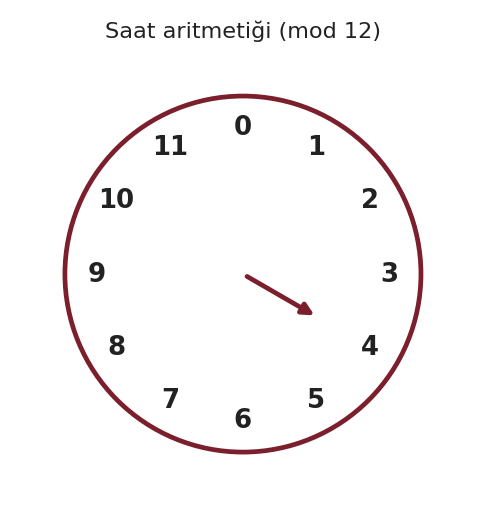
\includegraphics[width=0.56\linewidth]{figs/clock_mod.png}
\caption{Saat aritmetiği: mod 12 döngüsü.}
\end{figure}

\section{İleri Örnekler: Üs Alma, Ters Eleman ve Sistemler}

Kongrüansların gücü, büyük hesapları küçük döngülere indirgemesinde ortaya çıkar. Aşağıdaki örnekler modüler üs alma, ters eleman ve kongrüans sistemlerini gösterir.

\begin{tcolorbox}[bookbox,colback=cEx]\textbf{\textsf{\textcolor{cAcc}{Örnek.}}}\quad \textbf{Büyük üs. }10¹⁰⁰’ün 7’ye bölümünden kalan nedir? 10 ≡ 3 (mod 7) ve 3’ün kuvvetleri mod 7’de 3, 2, 6, 4, 5, 1 diye 6 adımda bir tekrarlar. 100 = 6·16 + 4 olduğundan 10¹⁰⁰ ≡ 3¹⁰⁰ ≡ 3⁴ ≡ 4 (mod 7). Kalan 4’tür — yüz basamaklı sayıyı hiç yazmadan.\end{tcolorbox}

\begin{tcolorbox}[bookbox,colback=cEx]\textbf{\textsf{\textcolor{cAcc}{Örnek.}}}\quad \textbf{11’e bölünebilme. }10 ≡ −1 (mod 11) olduğundan bir sayı, rakamlarının dönüşümlü (alternating) toplamına denktir. Örneğin 918082: 2 − 8 + 0 − 8 + 1 − 9 = −22 ≡ 0 (mod 11), yani 918082 sayısı 11’e bölünür.\end{tcolorbox}

\begin{tcolorbox}[bookbox,colback=cEx]\textbf{\textsf{\textcolor{cAcc}{Örnek.}}}\quad \textbf{Lineer kongrüans. }3x ≡ 4 (mod 5) çözülür: 3’ün mod 5 tersi 2’dir (çünkü 3·2 = 6 ≡ 1). İki tarafı 2 ile çarparsak x ≡ 8 ≡ 3 (mod 5). Denetim: 3·3 = 9 ≡ 4 ✓. Ters eleman ancak gcd(3, 5) = 1 olduğu için vardır.\end{tcolorbox}

\begin{tcolorbox}[bookbox,colback=cEx]\textbf{\textsf{\textcolor{cAcc}{Örnek.}}}\quad \textbf{Kongrüans sistemi (Çin Kalan Teoremi’nin önizlemesi). }x ≡ 2 (mod 3) ve x ≡ 3 (mod 5) sistemini sağlayan x, mod 15’te tek bir sınıftır: x ≡ 8 (mod 15). Denetim: 8 ≡ 2 (mod 3) ve 8 ≡ 3 (mod 5) ✓. Modüller aralarında asal olduğunda çözüm daima vardır ve çarpımları modunda tektir.\end{tcolorbox}

\begin{tcolorbox}[bookbox,colback=cMis]\textbf{\textsf{\textcolor{cAcc}{Yaygın Kavram Yanılgıları}}}\quad \textbf{“a ≡ b (mod n) ise a = b’dir.” — }Kongrüans eşitlik değildir; a ile b yalnızca aynı kalanı verir. 8 ≡ 3 (mod 5) doğrudur ama 8 ≠ 3.\par\medskip{}\textbf{“Kongrüansta her iki tarafı bölebilirim.” — }Sadeleştirme yalnızca bölünen sayı ile modül aralarında asalsa geçerlidir. 2·3 ≡ 2·0 (mod 6) iken 3 ≢ 0 (mod 6).\par\medskip{}\textbf{“aᵏ ≡ (a mod n)ᵏ’yı doğrudan hesaplarım, üssü de küçültürüm.” — }Taban mod n’e indirgenebilir, ama üs öyle indirgenemez; üs için kuvvetlerin döngüsü (ya da Euler teoremi) kullanılır.\par\medskip{}\textbf{“Her a’nın mod n tersi vardır.” — }Ters ancak gcd(a, n) = 1 iken vardır. Örneğin 2’nin mod 4 tersi yoktur.\par\medskip{}\textbf{“Negatif sayıların modu tanımsızdır.” — }Tanımlıdır: −3 ≡ 2 (mod 5), çünkü −3 + 5 = 2. Kalan daima 0 ile n − 1 arasında seçilir.\end{tcolorbox}

\section{Uygulama ve Eğitime Yansıma}

Modüler aritmetik gündelik teknolojinin görünmez altyapısıdır. Sağlama basamakları (ISBN, kredi kartlarında Luhn algoritması, TC kimlik numarası) hataları yakalamak için kongrüans kullanır; karma (hash) fonksiyonları ve rastgele sayı üreteçleri mod işlemiyle çalışır. En çarpıcı uygulama açık anahtarlı şifrelemedir (RSA): mesaj bir modül altında üs alınarak şifrelenir ve yalnızca ‘ters üssü’ bilen çözebilir.

Eğitim açısından modüler aritmetik, öğrenciye ‘eşitlik’ ile ‘denklik’ farkını en somut biçimde yaşatır ve soyut cebire (ℤₙ) yumuşak bir giriş sağlar. Saat aritmetiği ve haftanın günleri gibi tanıdık örnekler, konuyu günlük deneyime bağlayarak van Hiele düzeylerinde görsel/işlemsel düzeyden başlamayı kolaylaştırır.

\section{Yüksek Lisans Derinleştirmesi: ℤₙ Halkası ve Fermat–Euler}

Kongrüans sınıfları ℤₙ = \{[0], [1], …, [n − 1]\} kümesini oluşturur ve üzerindeki iyi tanımlı toplama–çarpma ile ℤₙ bir değişmeli halka olur. Bu halkanın çarpımsal tersi olan elemanları (birimler) tam olarak modülle aralarında asal olan sınıflardır; bunlar (ℤ/nℤ)* birimler grubunu oluşturur ve eleman sayısı Euler’in φ(n) fonksiyonuyla verilir. n asal olduğunda her sıfırdan farklı sınıfın tersi vardır, yani ℤₙ bir cisim (alan) olur.

Bu yapı iki klasik teoremi doğurur. Fermat’ın küçük teoremi: p asal ve gcd(a, p) = 1 ise aᵖ⁻¹ ≡ 1 (mod p). Onun genellemesi Euler teoremi: gcd(a, n) = 1 ise a\textasciicircum{}φ(n) ≡ 1 (mod n). Bu sonuçlar, ‘büyük üs’ örneğindeki döngüsel davranışın neden kaçınılmaz olduğunu açıklar: birimler grubunun sonlu olması, kuvvetlerin er geç tekrar 1’e dönmesini garanti eder.

RSA şifrelemesi tam da bu teoremlere dayanır: iki büyük asalın çarpımı n = pq alınır, şifreleme üssü e ve çözme üssü d, ed ≡ 1 (mod φ(n)) olacak biçimde seçilir; Euler teoremi sayesinde (mᵉ)ᵈ ≡ m (mod n) olur ve mesaj geri elde edilir. Güvenlik, n’i çarpanlarına ayırmanın (yani φ(n)’i bulmanın) pratikte çok zor olmasına dayanır. Böylece Bölüm~\ref{chap:kongruanslar}’nin soyut kongrüans cebri, doğrudan çağdaş güvenli iletişimin temeline bağlanır.

\section{Sayılar Kuramından Klasik Sonuçlar}

Kongrüans dili, sayılar kuramının pek çok klasik sonucunu erişilebilir kılar. Aşağıdaki örnekler bu gücü gösterir ve bölüm boyunca kurulan araçların nasıl bir araya geldiğini sergiler.

\begin{tcolorbox}[bookbox,colback=cEx]\textbf{\textsf{\textcolor{cAcc}{Örnek.}}}\quad \textbf{Euler φ hesabı. }φ(n), n ile aralarında asal olan 1 ≤ k ≤ n sayılarının adedidir. Örneğin φ(12) = 4 (bunlar 1, 5, 7, 11). Asal p için φ(p) = p − 1; aralarında asal m, n için φ(mn) = φ(m)φ(n). Bu fonksiyon, birimler grubunun büyüklüğünü verdiği için Euler teoreminin merkezindedir.\end{tcolorbox}

\begin{tcolorbox}[bookbox,colback=cEx]\textbf{\textsf{\textcolor{cAcc}{Örnek.}}}\quad \textbf{Çin Kalan Teoremi (tam çözüm). }x ≡ 2 (mod 3), x ≡ 3 (mod 5), x ≡ 2 (mod 7) sistemini çözelim. İlk iki denklik x ≡ 8 (mod 15) verir; buna x ≡ 2 (mod 7) eklenince x ≡ 23 (mod 105) bulunur. Denetim: 23 = 3·7 + 2, 23 = 4·5 + 3, 23 = 7·3 + 2. Modüller ikişer aralarında asal olduğundan çözüm, çarpımları olan 105 modunda tektir.\end{tcolorbox}

\begin{tcolorbox}[bookbox,colback=cEx]\textbf{\textsf{\textcolor{cAcc}{Örnek.}}}\quad \textbf{Wilson teoremi. }p asal ise (p − 1)! ≡ −1 (mod p). Örneğin p = 5 için 4! = 24 ≡ −1 (mod 5). Bu, bir sayının asallığını (verimsiz de olsa) kongrüansla sınayan zarif bir ölçüttür ve modüler çarpımın grup yapısını sergiler.\end{tcolorbox}

Dokuza atma (casting out nines), bu fikirlerin gündelik bir uygulamasıdır: bir çarpma işleminin doğruluğu, tarafların rakam toplamları mod 9’da karşılaştırılarak hızlıca sınanabilir; çünkü 10 ≡ 1 (mod 9), dolayısıyla her sayı rakam toplamına denktir. Bu yöntem her hatayı yakalamayı garanti etmez ama pek çok hatayı anında görünür kılar ve öğrenciye kongrüansın pratik değerini somutlaştırır.

Bu örnekler, Bölüm~\ref{chap:kongruanslar}’nin yalnızca soyut bir cebir alıştırması olmadığını ortaya koyar: Gauss’un icat ettiği dil, hem klasik sayılar kuramının derin teoremlerini hem de bilgisayar çağının şifreleme altyapısını taşıyacak kadar güçlüdür. Öğretmen adayı için buradaki ders, ‘saf’ ile ‘uygulamalı’ matematiğin çoğu zaman aynı fikrin iki yüzü olduğudur; kalanların basit aritmetiği, doğru ışıkta bakıldığında modern güvenli iletişimin temeline uzanır.

\section{Hızlı Üs Alma ve Bir RSA Örneği}

Modüler aritmetiğin pratik gücü, ‘tekrarlı kareleme’ (repeated squaring) yöntemiyle büyük üsleri hızla hesaplayabilmesinde ortaya çıkar. Fikir basittir: üssü ikili tabanda düşünüp tabanın karelerini birbiriyle çarparız; böylece n’inci kuvvet için n çarpma yerine yalnızca log₂n dolayında çarpma yeter.

\begin{tcolorbox}[bookbox,colback=cEx]\textbf{\textsf{\textcolor{cAcc}{Örnek.}}}\quad \textbf{Tekrarlı kareleme. }3¹³ mod 100 hesaplayalım. 13 = 8 + 4 + 1 olduğundan 3¹³ = 3⁸ · 3⁴ · 3¹. Kareleri sırayla bulalım: 3² = 9, 3⁴ = 81, 3⁸ = 81² = 6561 ≡ 61 (mod 100). Şimdi 3¹³ ≡ 61 · 81 · 3 (mod 100): 61 · 81 = 4941 ≡ 41, sonra 41 · 3 = 123 ≡ 23. Demek ki 3¹³ ≡ 23 (mod 100) — on üç çarpma yerine birkaç kareleme ile.\end{tcolorbox}

Bu yöntem, açık anahtarlı şifrelemenin (RSA) hesaplanabilir olmasının anahtarıdır: gerçek uygulamada üsler yüzlerce basamaklıdır ve yalnızca tekrarlı kareleme sayesinde makul sürede hesaplanır. Aşağıda RSA’nın çekirdek fikrini küçük sayılarla baştan sona izleyelim.

\begin{tcolorbox}[bookbox,colback=cEx]\textbf{\textsf{\textcolor{cAcc}{Örnek.}}}\quad \textbf{RSA (küçük örnek). }İki asal seçelim: p = 3, q = 11, böylece n = pq = 33 ve φ(n) = (p − 1)(q − 1) = 2 · 10 = 20. Şifreleme üssü olarak gcd(e, 20) = 1 sağlayan e = 3’ü alalım; çözme üssü d ise 3d ≡ 1 (mod 20) denkleminden d = 7’dir (çünkü 3 · 7 = 21 ≡ 1). Açık anahtar (n, e) = (33, 3), gizli anahtar (n, d) = (33, 7).\end{tcolorbox}

\begin{tcolorbox}[bookbox,colback=cEx]\textbf{\textsf{\textcolor{cAcc}{Örnek.}}}\quad \textbf{Şifreleme ve çözme. }m = 2 mesajını şifreleyelim: c = mᵉ mod n = 2³ = 8 (mod 33). Çözmek için c\textasciicircum{}d mod n = 8⁷ (mod 33) hesaplanır. Tekrarlı karelemeyle: 8² = 64 ≡ 31, 8⁴ ≡ 31² = 961 ≡ 4, dolayısıyla 8⁷ = 8⁴ · 8² · 8 ≡ 4 · 31 · 8 = 992 ≡ 2 (mod 33). Başlangıçtaki m = 2 mesajı geri elde edildi. ✓\end{tcolorbox}

Bu örnek RSA’nın neden çalıştığını da somutlaştırır: ed ≡ 1 (mod φ(n)) seçildiğinden, Euler teoremi (Bölüm~\ref{chap:kongruanslar}) gereği (mᵉ)ᵈ = m\textasciicircum{}\{ed\} ≡ m (mod n) olur. Güvenlik ise şuna dayanır: açık anahtardan (n, e) gizli anahtarı (d) bulmak için φ(n) gerekir; φ(n)’i bulmak da n’i asal çarpanlarına (p ve q) ayırmayı gerektirir. Küçük sayılarda bu kolaydır, ama yüzlerce basamaklı n için pratikte çözülemez zorluktadır.

Böylece Gauss’un iki yüzyıl önce icat ettiği kongrüans dili, bugün internetteki güvenli iletişimin (bankacılık, mesajlaşma, dijital imza) matematiksel temelini oluşturur. Öğretmen adayı için bu, ‘neden soyut sayılar kuramı öğreniyoruz?’ sorusuna verilebilecek en çarpıcı yanıtlardan biridir: en saf matematik, çoğu zaman en somut teknolojinin kalbinde yatar.

\begin{tcolorbox}[bookbox,colback=cDef]\textbf{\textsf{\textcolor{cAcc}{Tarihsel Not}}}\quad Carl Friedrich Gauss, kongrüans gösterimini içeren başyapıtı Disquisitiones Arithmeticae’yi 1801’de, henüz yirmi dört yaşındayken yayımladı. Eser, dağınık sayı-kuramı gözlemlerini tek bir sistemli çerçevede topladı ve modüler aritmetiği bağımsız bir disiplin hâline getirdi. İlginç bir tarihsel bağ: Fermat’ın küçük teoremi, Pierre de Fermat tarafından 1640’ta bir mektupta ispatsız dile getirilmiş, ilk yayımlanan ispatı ise Euler’den gelmiştir. Bu teorem, iki yüzyıl sonra RSA şifrelemesinin çekirdeği olacaktı.\end{tcolorbox}

\section{Modüler Aritmetiği Görmek: Döngüler ve Kontrol Basamakları}

Modüler aritmetikte kuvvetler ve katlar sonunda kendini tekrar eder; çünkü yalnızca sonlu sayıda kalan vardır. Bu tekrarı bir çember üzerinde çizmek, Fermat teoreminin ve ‘üreteç’ kavramının neden işlediğini sezdirir.

\begin{figure}[htbp]
\centering
\begin{tikzpicture}[v/.style={circle,draw=bar,fill=white,line width=.8pt,minimum size=6.5mm,font=\sffamily\small},>={Stealth[length=5pt]}]
\begin{scope}
\foreach \k in {0,...,6}{\node[v] (a\k) at ({90-360/7*\k}:1.6) {\k};}
\foreach \x/\y in {1/3,3/2,2/6,6/4,4/5,5/1}{\draw[->,acc,line width=.9pt] (a\x) to[bend left=12] (a\y);}
\draw[->,mid,line width=.8pt] (a0) edge[loop above,looseness=6] (a0);
\node[small lbl,anchor=north] at (0,-2.05) {$x\mapsto 3x \pmod 7$\\tek döngü: $1\to3\to2\to6\to4\to5\to1$};
\end{scope}
\begin{scope}[xshift=5.2cm]
\foreach \k in {0,...,6}{\node[v] (b\k) at ({90-360/7*\k}:1.6) {\k};}
\foreach \x/\y in {1/2,2/4,4/1}{\draw[->,warm,line width=.9pt] (b\x) to[bend left=12] (b\y);}
\foreach \x/\y in {3/6,6/5,5/3}{\draw[->,grn,line width=.9pt] (b\x) to[bend left=12] (b\y);}
\draw[->,mid,line width=.8pt] (b0) edge[loop above,looseness=6] (b0);
\node[small lbl,anchor=north] at (0,-2.05) {$x\mapsto 2x \pmod 7$\\iki döngü: $1\to2\to4\to1$ ve $3\to6\to5\to3$};
\end{scope}
\end{tikzpicture}
\caption{Mod 7’de 3 ile ve 2 ile çarpmanın kalanlar üzerindeki etkisi. 3 ile çarpma sıfırdan farklı altı kalanı tek bir döngüde dolaşır (3 bir \emph{üreteçtir}); 2 ile çarpma ise iki ayrı üçlü döngü oluşturur. Her iki durumda da döngü uzunluğu 6’yı böler — Fermat teoreminin ($a^{6}\equiv1$) görsel karşılığı.}
\end{figure}

\begin{table}[htbp]
\centering\small
\renewcommand{\arraystretch}{1.25}
\begin{tabular}{lcccccc}
\toprule
$k$ & 1 & 2 & 3 & 4 & 5 & 6\\
\midrule
$2^k \bmod 7$ & 2 & 4 & \textbf{1} & 2 & 4 & 1\\
$3^k \bmod 7$ & 3 & 2 & 6 & 4 & 5 & \textbf{1}\\
\bottomrule
\end{tabular}
\caption{Kuvvetlerin kalanları. 2’nin kuvvetleri 3 adımda, 3’ün kuvvetleri 6 adımda başa döner. Buradan örneğin $2^{100}=2^{3\cdot33+1}\equiv2 \pmod 7$ hemen okunur.}
\end{table}

\begin{ornek}[\textbf{Kontrol basamağı: ISBN-10.}]
Eski on haneli ISBN numaralarında $a_1a_2\cdots a_{10}$ rakamları için
\[
10a_1+9a_2+8a_3+\cdots+2a_9+1\cdot a_{10}\equiv0 \pmod{11}
\]
koşulu aranır; son hane bu koşulu sağlayacak biçimde seçilir (gerekirse 10 yerine ‘X’ yazılır). 0-306-40615-2 numarası için toplam
\[
0+27+0+42+24+0+24+3+10+2=132=12\cdot11\equiv0 \pmod{11}
\]
olduğundan numara geçerlidir. Neden 11? Tek bir rakam hatası toplamı $c\cdot d$ kadar değiştirir ($c$ ağırlık, $d$ hata); 11 asal ve $1\le c,d\le10$ olduğundan bu değişim 11’e bölünemez, hata mutlaka yakalanır. Komşu iki rakamın yer değiştirmesi de toplamı $\pm(a_i-a_{i+1})$ kadar değiştirir ve aynı nedenle yakalanır. Modülün asal olması, sıfır bölen bulunmaması demektir — aşağıdaki yanılgı kutusuyla karşılaştırın.
\end{ornek}

\begin{ornek}[\textbf{İki koşulu birden sağlamak.}]
3’e bölündüğünde 2, 5’e bölündüğünde 3 kalanını veren sayıları arayalım. $x\equiv3\pmod5$ koşulunu sağlayanlar $3,8,13,18,23,\dots$ dizisidir; bunların 3’e göre kalanları $0,2,1,0,2,\dots$ biçiminde döner. İlk uygun değer 8’dir ve 3 ile 5 aralarında asal olduğundan çözümler tam olarak $x\equiv8\pmod{15}$ sınıfıdır. Bu, \emph{Çin kalan teoreminin} en küçük örneğidir: aralarında asal modüller için eşzamanlı kongrüansların çözümü vardır ve çarpım modülüne göre tektir — varlık ve teklik sorularının modüler aritmetikteki biçimi.
\end{ornek}

\begin{yanilgi}[Yaygın Kavram Yanılgıları]
\textbf{‘$ab\equiv0$ ise $a\equiv0$ ya da $b\equiv0$’dır.’} — Mod 6’da $2\cdot3=6\equiv0$ ama ne 2 ne 3 sıfırdır. Bu özellik ancak modül asal olduğunda geçerlidir.

\smallskip
\textbf{‘Her iki tarafı aynı sayıya bölebilirim.’} — $2x\equiv2\pmod6$ kongrüansında 2’ye ‘bölerek’ $x\equiv1$ yazmak, $x=4$ çözümünü kaybettirir ($2\cdot4=8\equiv2$). Doğru kural: $\gcd(c,n)=d$ ise $cx\equiv cy\pmod n\iff x\equiv y\pmod{n/d}$; burada $x\equiv1\pmod3$.

\smallskip
\textbf{‘$a\equiv b\pmod n$ ise $2^a\equiv2^b\pmod n$’dir.’} — Üsler aynı modülde indirgenemez: $4\equiv1\pmod3$ ama $2^4=16\equiv1$, $2^1=2$. Üsler, kuvvetlerin döngü uzunluğuna göre indirgenir (Fermat–Euler).
\end{yanilgi}

\begin{sinif}[Sınıfta · Haftanın günü]
‘Bugün salı. 100 gün sonra hangi gün olur? $10^{10}$ gün sonra?’ Birinci soru $100\equiv2\pmod7$ ile kolayca çözülür. İkincisi için öğrenciler $10\equiv3\pmod7$ gözleminden sonra yukarıdaki $3^k$ tablosunu kullanarak $3^{10}=3^{6}\cdot3^4\equiv4\pmod7$ bulur: dört gün sonrası, yani cumartesi. Etkinlik, ‘sayıyı hesaplamadan kalanını bulmak’ fikrini — bölümün ana düşüncesini — somutlaştırır.
\end{sinif}

\section*{Alıştırmalar}

\reviewitem{1}{7¹⁰⁰ sayısının 5’e bölümünden kalanı bulun.}

\reviewitem{2}{3x ≡ 1 (mod 7) denklemini çözün ve 3’ün mod 7 tersini belirtin.}

\reviewitem{3}{Bir sayının 11’e bölünebilme kuralını, 10 ≡ −1 (mod 11) kongrüansını kullanarak gerekçelendirin.}

\reviewitem{4}{φ(36) değerini hesaplayın (çarpımsallık özelliğini kullanabilirsiniz).}

\reviewitem{5}{RSA örneğini p = 5, q = 11 ile tekrarlayın: n ve φ(n)’i bulun, uygun bir e seçin ve buna karşılık gelen d’yi hesaplayın.}

\section*{Bölüm Özeti}

\begin{itemize}\setlength{\itemsep}{2pt}\setlength{\parskip}{0pt}
\item a ≡ b (mod n) ⇔ n | (a − b); bir denklik bağıntısıdır.
\item Kongrüans toplama ve çarpma ile uyumludur; bu ℤₙ aritmetiğini kurar.
\item Bölünebilme kuralları ve döngüsel sayma kongrüansların uygulamalarıdır.
\end{itemize}

\section*{Gözden Geçirme Soruları}

\reviewitem{1}{7 | (a − b) uyumunu kullanarak 10¹⁰⁰’ün 7’ye bölümünden kalanı bulunuz (yaklaşımınızı açıklayın).}

\reviewitem{2}{Çıkarmanın da kongrüansla uyumlu olduğunu gösteriniz.}

\section*{Çoktan Seçmeli Sorular}

\mcqq{1}{a ≡ b (mod n) ne demektir?}

\mcqo{A}{a = b}

\mcqo{B}{n | (a − b)}

\mcqo{C}{a | (n − b)}

\mcqo{D}{b | (a − n)}

\mcqa{B}{a≡b (mod n): n, a−b’yi böler.}

\mcqq{2}{Kongrüans ℤ üzerinde ne tür bir bağıntıdır?}

\mcqo{A}{Sıralama}

\mcqo{B}{Denklik}

\mcqo{C}{Fonksiyon}

\mcqo{D}{Ters simetrik}

\mcqa{B}{Kongrüans ℤ üzerinde bir denklik bağıntısıdır.}

\mcqq{3}{9’a bölünebilme kuralı hangi kongrüansa dayanır?}

\mcqo{A}{10 ≡ 0 (mod 9)}

\mcqo{B}{10 ≡ 1 (mod 9)}

\mcqo{C}{9 ≡ 1 (mod 10)}

\mcqo{D}{10 ≡ −1 (mod 9)}

\mcqa{B}{10≡1 (mod 9) olduğundan sayı, rakam toplamına denktir.}

\mcqq{4}{17 ≡ ? (mod 5)}

\mcqo{A}{0}

\mcqo{B}{1}

\mcqo{C}{2}

\mcqo{D}{3}

\mcqa{C}{17 = 3·5 + 2, kalan 2.}

\mcqq{5}{a ≡ a′ ve b ≡ b′ (mod n) ise a + b ≡ ?}

\mcqo{A}{a′ + b′}

\mcqo{B}{a′ − b′}

\mcqo{C}{a′b′}

\mcqo{D}{a′}

\mcqa{A}{Toplama kongrüansla uyumludur: a+b ≡ a′+b′.}

\mcqq{6}{a ≡ a′ ve b ≡ b′ (mod n) ise a·b ≡ ?}

\mcqo{A}{a′ + b′}

\mcqo{B}{a − b}

\mcqo{C}{a′b′}

\mcqo{D}{0}

\mcqa{C}{Çarpma kongrüansla uyumludur: ab ≡ a′b′.}

\mcqq{7}{25 ≡ ? (mod 7)}

\mcqo{A}{1}

\mcqo{B}{2}

\mcqo{C}{3}

\mcqo{D}{4}

\mcqa{D}{25 = 3·7 + 4, kalan 4.}

\mcqq{8}{Kongrüansın yansıma özelliği (a ≡ a) neye dayanır?}

\mcqo{A}{n | a}

\mcqo{B}{n | 0}

\mcqo{C}{n | 1}

\mcqo{D}{a | n}

\mcqa{B}{a−a = 0 ve n|0 olduğundan a≡a.}

\mcqq{9}{−3 ≡ ? (mod 5)}

\mcqo{A}{−3}

\mcqo{B}{3}

\mcqo{C}{2}

\mcqo{D}{4}

\mcqa{C}{−3 + 5 = 2, yani −3 ≡ 2 (mod 5).}

\mcqq{10}{Bir sayının 3’e bölünebilmesi için ölçüt nedir?}

\mcqo{A}{Son rakamı 3’tür}

\mcqo{B}{Rakamları toplamı 3’e bölünür}

\mcqo{C}{Çifttir}

\mcqo{D}{Son iki rakamı 3’e bölünür}

\mcqa{B}{10≡1 (mod 3) olduğundan rakam toplamı 3 için de ölçüttür.}

\mcqq{11}{Saat aritmetiği hangi modda çalışır?}

\mcqo{A}{mod 7}

\mcqo{B}{mod 10}

\mcqo{C}{mod 12}

\mcqo{D}{mod 60}

\mcqa{C}{Saat, 12 modunda döngüseldir.}

\mcqq{12}{Haftanın günleri hangi modda döngüseldir?}

\mcqo{A}{mod 12}

\mcqo{B}{mod 7}

\mcqo{C}{mod 24}

\mcqo{D}{mod 30}

\mcqa{B}{Günler 7 modunda tekrarlanır.}

\mcqq{13}{ℤₙ neyi mümkün kılar?}

\mcqo{A}{Sonsuz işlem}

\mcqo{B}{Sonlu bir küme üzerinde tutarlı toplama ve çarpma}

\mcqo{C}{Sıralama}

\mcqo{D}{Her zaman bölme}

\mcqa{B}{İşlemlerle uyum, ℤₙ üzerinde tutarlı aritmetiği kurar.}

\mcqq{14}{Kongrüansın toplama ile uyumu neye dayanır?}

\mcqo{A}{Çarpmaya}

\mcqo{B}{n | (a − a′) ve n | (b − b′) ⇒ n | toplam farkı}

\mcqo{C}{Sıralamaya}

\mcqo{D}{Fermat teoremine}

\mcqa{B}{(a−a′)+(b−b′) farkının bölünmesi toplama uyumunu verir.}

\mcqq{15}{100 ≡ ? (mod 9)}

\mcqo{A}{0}

\mcqo{B}{1}

\mcqo{C}{2}

\mcqo{D}{9}

\mcqa{B}{100 = 11·9 + 1, kalan 1.}

\mcqq{16}{Fermat’ın küçük teoremi (p asal) ne der?}

\mcqo{A}{a\textasciicircum{}p ≡ 0 (mod p)}

\mcqo{B}{a\textasciicircum{}p ≡ a (mod p)}

\mcqo{C}{a ≡ p}

\mcqo{D}{a² ≡ 1 (mod p)}

\mcqa{B}{Fermat: p asalsa a\textasciicircum{}p ≡ a (mod p).}

\mcqq{17}{a ≡ b (mod n) ise a ve b’nin n’ye bölümünden kalanları nasıldır?}

\mcqo{A}{Farklıdır}

\mcqo{B}{Eşittir}

\mcqo{C}{Toplamı n’dir}

\mcqo{D}{Çarpımı 0’dır}

\mcqa{B}{Aynı sınıftaki sayılar aynı kalanı verir.}

\mcqq{18}{12 ≡ 0 (mod n) eşitliği aşağıdaki hangi n için doğrudur?}

\mcqo{A}{n = 5}

\mcqo{B}{n = 7}

\mcqo{C}{n = 3}

\mcqo{D}{n = 8}

\mcqa{C}{3 | 12 olduğundan 12 ≡ 0 (mod 3).}

\mcqq{19}{Kongrüans neden “yapı koruyan” bir muhakeme örneğidir?}

\mcqo{A}{Sayıları büyütür}

\mcqo{B}{Ayrıntıyı atarken toplama–çarpma yapısını korur}

\mcqo{C}{Yalnızca bilgi kaybettirir}

\mcqo{D}{İşe yaramaz}

\mcqa{B}{Ayrıntıyı atarken toplama-çarpma yapısını korur.}

\mcqq{20}{7 | (a − b) bağıntısında [0] denklik sınıfı nedir?}

\mcqo{A}{Tek sayılar}

\mcqo{B}{7’nin katları}

\mcqo{C}{Asal sayılar}

\mcqo{D}{Tüm ℤ}

\mcqa{B}{[0], farkı 7’ye bölünenler, yani 7’nin katlarıdır.}


\clearpage

\clearpage